\documentclass[a4paper,12pt]{scrartcl}
\usepackage{exercice_sheet}

%\trait
%\section*{}
%\exo{}
%\question{}
%\subquestion{}


\date{}

\newcommand{\classe}{CG}
\newcommand{\typedevoir}{BTS blanc} 
\newcommand{\duree}{2 heures}

\renewcommand{\hascorrection}{0}


% Title Page
\title{\textbf{\typedevoir{} -- \classe{}\writecorrword{} \\
Mathématiques}} 

\author{Durée : \duree{}}


\begin{document}

\maketitle

\exo{Mathématiques financières}

Un capital placé à 9\% pendant une certaine période a acquis une valeur de 435 000\euro{}. Placé à 10\% pendant un an de moins, ce même capital aurait produit des intérêts de 120 000\euro{}.

\question{}
Exprimer le capital $(V_0)$ en fonction de la durée $n$ pour le premier placement.

\correction{
$V_n = V_0(1+ni)$

$V_0 = \dfrac{435000}{1+0.09n}$
}

\question{}
Exprimer le capital $(V_0)$ en fonction de la durée $n$ pour le deuxième placement.

\correction{
$I_n=V_0 ni$

$120 000 = V_0 \times (n-1) \times 0.1$

$V_0 = \dfrac{1 200 000}{n-1}$
}

\question{}
Déterminer la durée $n$ du premier placement.

\correction{
$ 435 000 (n-1)=1 200 000 (1+0.09n)$ 

$435000n - 435000 = 1200000 + 108000n$

$435000n - 108000n = 1200000 + 435000$ 

$N = \dfrac{1635000}{327000} = 5$ 
}

\question{}
Déterminer la valeur du capital placé.

\correction{
Reprise de la question 2 donc 1200000 / 4 = 300000 \euro{} 
}

Données: 

$V_n = V_0(1+n \cdot i)$ et $I_n = V_0 \cdot n \cdot i$ 

\exo{Étude de fonction}

Soit $f$ la fonction définie sur $[6; 30]$ par $f(x) = \dfrac{1}{2}x^2 - 36 \ln x + 150$.  

On note $\mathcal{C}$ la courbe représentative de $f$ dans un repère orthogonal $\left(O ; \overrightarrow{i} ; \overrightarrow{j} \right)$. On prendra comme unités graphiques : 1 cm pour 5 sur l'axe des abscisses et un centimètre pour 100 sur l'axe des ordonnées.
 
 \question{Dérivée}
 
 \subquestion{}
 Montrer que, pour tout nombre réel $x$ de $[6;30]$,
 
\begin{equation*}
f'(x) = \dfrac{(x+6)(x-6)}{x}
\end{equation*}

\correction{
\begin{equation*}
f'(x) = x - \dfrac{36}{x} = \dfrac{x^2 - 36}{x} = \dfrac{(x+6)(x-6)}{x}
\end{equation*}
}
 
 \subquestion{}
 Étudier le signe de $f'(x)$ lorsque $x$ varie dans $[6;30]$.

\correction{
Sur $[6;30]$, $x>0$, $x+6>0$ et $x-6 \geqslant 0$, donc $f'(x) \geqslant 0$ sur $[6;30]$.
}
 
 \subquestion{}
 En déduire la tableau de variation de $f$ sur $[6;30]$.

\correction{
\begin{center}
\begin{tikzpicture}
   \tkzTabInit{$x$ / 1 , $f(x)$ / 2}{$6$, $30$}
   \tkzTabVar{-/ $103$, +/ $478$}
\end{tikzpicture}
\end{center}
}
 
 \question{Tracé de la courbe}
 
 \subquestion{}
Compléter, après l'avoir reproduit sur la copie, le tableau de valeurs suivant dans lequel les valeurs approchées sont à arrondir à l'unité.

\begin{center}
\begin{tabular}{|c|c|c|c|c|c|c|}
\hline
$x$    & 6 & 10 & 15 & 20 & 25 & 30 \\ \hline
$f(x)$ & \hspace{15mm}  &  \hspace{15mm}  &  \hspace{15mm}  &  \hspace{15mm}  &  \hspace{15mm}  &  \hspace{15mm}  \\ \hline
\end{tabular}
\end{center}

\correction{
\begin{center}
\begin{tabular}{|c|c|c|c|c|c|c|}
\hline
$x$    & 6    & 10    & 15   & 20  & 25  & 30 \\ \hline
$f(x)$ & 103  &  117  & 165  & 242 & 347 & 478 \\ \hline
\end{tabular}
\end{center}
}

 
 \subquestion{}
 Tracer la courbe $\mathcal{C}$ dans un repère sur la copie. 

\correction{
\begin{center}
\simpleplot{6}{30}{\x}{0.5*(\x)^2 - 36*ln(\x) + 150}{$\mathcal{C}_f$}{1}
\end{center}
}  

\exo{Suites}
On place une somme d'argent notée $S_0$ au taux annuel de 5.5\%, ce placement étant à intérêts composés.

Pour tout entier naturel $n$, $S_n$ désigne le capital disponible au bout de $n$ années.

\question{}
Justifier que la suite $(S_n)$ est géométrique. Préciser la raison de cette suite.

\correction{
$S_{n+1} = S_n \times 1.055$ donc $(S_n)$ est géométrique de raison 1.055.
}

\question{}
Exprimer $S_n$ en fonction de $S_0$ et de $n$.

\correction{
On en déduit donc $S_n = S_0 \times 1.055^n$. 
}

\question{}
On place 1000\euro{} en 2019. Aucun transfert d'argent n'est fait après le placement. De combien dispose-t-on en 2030?

\correction{
La somme en 2019 correspondant $S_0$, on calcule $S_{11}$.

$S_{11} = 1000 \times 1.055^{11} = 1802.09$\euro{}.
}
 
 
\probleme{Probabilités}

\partie{Probabilités conditionnelles}

Pour contacter une compagnie d'assurances, deux possibilités sont offertes:

\begin{itemize}
\item se rendre en agence ;
\item à distance par téléphone.
\end{itemize}

Le responsable du pôle \og{}satisfaction client\fg{} décide de réaliser une enquête afin de savoir si les clients qui se rendent en agence ou qui contactent la compagnie par téléphone sont satisfaits de l'accueil.

À l'issue de l'enquête réalisée auprès de 1 000 clients, les résultats sont les suivants

\begin{itemize}
\item 380 se sont rendus en agence,
\item parmi les clients qui se sont rendus en agence, 93 \% se sont déclarés satisfaits de l'accueil,
\item parmi les clients qui ont téléphoné, 15 \% ont déclaré qu'ils n'étaient pas satisfaits de l'accueil.
\end{itemize}

On interroge au hasard un client.

On considère les évènements suivants :

$A$ : \og{}Le client s'est rendu en agence\fg{}

$S$ : \og{}Le client est satisfait de l'accueil\fg{}.

On rappelle que l'événement contraire de $A$ se note $\overline{A}$ , que la probabilité de l'évènement $A$ se note $P(A)$ et que la probabilité de l'événement $A$ sachant que l'événement $B$ est réalisé se note $P_B(A)$.

Dans toute cette partie, les probabilités seront arrondies à $10^{-4}$, si nécessaire.

\question{}
Donner la valeur des probabilités $P\left(\overline{A}\right)$, $P_A(S)$ et $P_{\overline{A}} \left(\overline{S}\right)$.

\correction{
$P\left(\overline{A}\right) = 1 - \dfrac{380}{1000} = 0.62$, 

$P_A(S) = 0.93$ (énoncé), 

$P_{\overline{A}} \left(\overline{S}\right) = 0.15$ (énoncé).
}


\question{}
L'arbre de probabilités donné en annexe à rendre avec la copie représente la situation. Compléter celui-ci.

\correction{
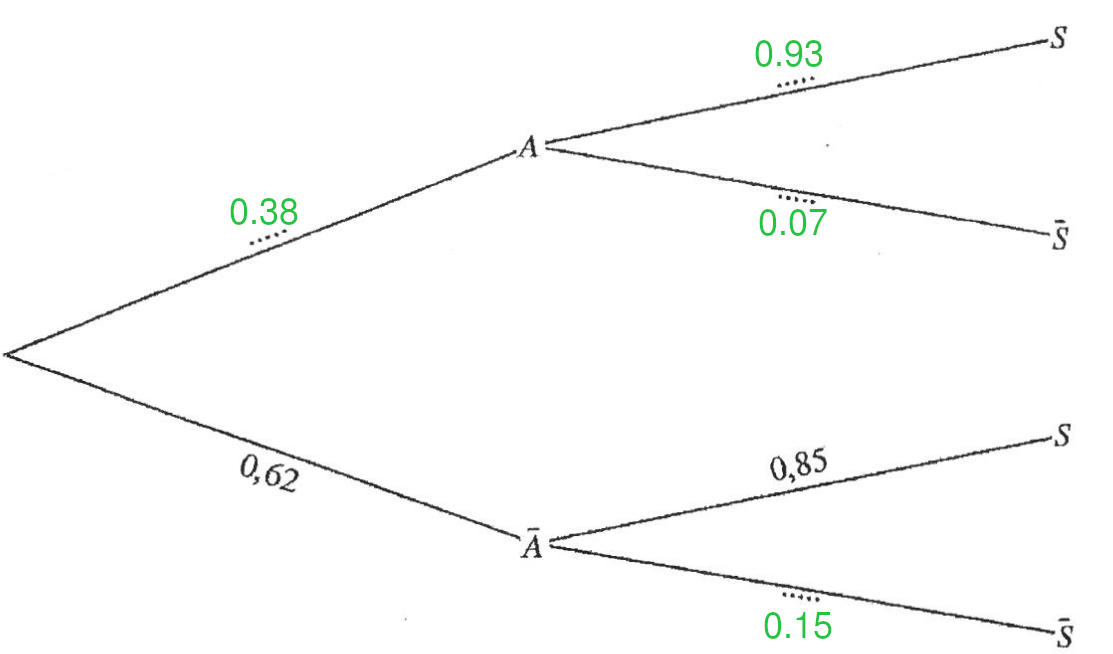
\includegraphics[width=\linewidth]{Arbuste_corr.png}
}


\question{}
Calculer la probabilité que le client se soit rendu en agence \textbf{et} qu'il ait été satisfait de l'accueil.

\correction{
Il s'agit de calculer $P(A \cap S) = P(A) \times P_A(S) = 0.38 \times 0.93 = 0.3534$.
}

\question{}
Montrer que la probabilité de $S$ est $0,8804$. 

\correction{
$P(S) = P(A \cap S) + P(\overline{A} \cap S) = 0.38 \times 0.93 + 0.62 \times 0.85 = 0.8804$.
}

\question{}
Le responsable a pour objectif qu'il y ait moins de 10 \% des clients non satisfaits par l'accueil. Cet objectif est-il atteint?

\correction{
Il y a environ 88\% de satisfaits donc environ 12\% d'insatisfaits. L'objectif n'est donc pas atteint. 
}

\question{}
Sachant que le client a été satisfait, quelle est la probabilité qu'il se soit rendu en agence?

\correction{
Il s'agit de calculer la probabilité $P_S(A)$. 

$P_S(A) = \dfrac{P(A \cap S)}{P(S)} = \dfrac{0.3534}{0.8804} = 0.4014$.
}

\partie{Loi binomiale}
Un employé prend au hasard 10 dossiers de sinistres de l'année en cours. Ce tirage est assimilé à un tirage avec remise car le nombre de dossiers est très grand.

On suppose que la probabilité que le coût du sinistre dépasse 1 000 euros est $0.84$.

Soit $Y$ la variable aléatoire qui, pour un lot de 10 dossiers pris au hasard, indique le nombre de dossiers du lot dont le coût est supérieur à 1 000 euros.

dans cette partie, les résultats seront arrondis à $10^{-3}$.

\question{}
Justifier que la variable aléatoire $Y$ suit une loi binomiale dont on donnera les paramètres.

\correction{
\begin{itemize}
\item $Y$ mesure le nombre de succès d'une suite d'épreuves ne comportant chacune que deux issues (succès ou échec). Ici, la probabilité de succès est $0.84$.
\item Toutes les épreuves sont identiques et indépendantes.
\item Le nombre d'épreuves est fixé à l'avance et est de $10$.
\end{itemize}

$Y$ suit donc une loi binomiale $\mathcal{B}(10;0.84)$.
}

\question{}
Calculer la probabilité que dans le lot prélevé par l'employé, tous les dossiers aient un coût supérieur à 1000 euros. 

\correction{
$P(Y=10) = C_{10}^{10} \times 0.84^{10} \times (1-0.84)^0 = 0.175$.
}

\question{}Calculer le probabilité que l'employé obtienne dans le lot prélevé au moins six dossiers dont le coût est supérieur à 1 000 euros. 

\correction{
$P(Y \geqslant 6) = 1 - P(Y \leqslant 5) = 0.987$.
}




\section*{Formulaire}

\section*{Dérivation}

\subsection*{Dérivées de fonctions usuelles}

\begin{center}

\begin{tabular}{|c|c|}
\hline 
\textbf{fonction $f$} & \textbf{fonction dérivée $f'$} \\ 
\hline 
$k$, $k \in \mathbb{R}$ & $0$ \\ 
\hline 
$x$ & $1$ \\ 
\hline 
$x^2$ & $2x$ \\ 
\hline 
$x^{\alpha}$, $\alpha \in \mathbb{Z}$ & $\alpha x^{\alpha - 1}$ \\ 
\hline 
$e^x$ & $e^x$ \\ 
\hline 
$\ln x$ & $\dfrac{1}{x}$ \\ 
\hline 
$\sqrt{x}$ & $\dfrac{1}{2\sqrt{x}}$ \\ 
\hline 
\end{tabular} 
\end{center}

\subsection*{Dérivées de produits, quotients, etc.}

\begin{center}
\begin{tabular}{|c|c|}
\hline 
\textbf{fonction $f$} & \textbf{fonction dérivée $f'$} \\ 
\hline 
$u+v$ & $u'+v'$ \\ 
\hline 
$ku$ & $ku'$ \\ 
\hline 
$u \times v$ & $u'v+uv'$ \\ 
\hline 
$\dfrac{u}{v}$ & $\dfrac{u'v-uv'}{v^2}$ \\ 
\hline 
$\dfrac{1}{u}$ & $-\dfrac{u'}{u^2}$ \\ 
\hline 
\end{tabular} 
\end{center}

% \subsection*{Dérivées de fonctions composées}
% 
% 
% \begin{center}
% \begin{tabular}{|c|c|}
% \hline 
% \textbf{fonction $f$} & \textbf{fonction dérivée $f'$} \\ 
% \hline 
% $v \circ u$ ou $v(u(x))$ & $u' \times v' \circ u $ ou $u'(x) \times v'(u(x))$ \\ 
% \hline 
% $e^u$ & $u'e^u$ \\ 
% \hline 
% $\ln u$ & $\dfrac{u'}{u}$ \\ 
% \hline 
% $u^\alpha$ & $\alpha u' u^{\alpha - 1}$ \\ 
% \hline 
% \end{tabular}
% \end{center}


\section*{Probabilités générales}

\begin{equation*}
 P(A \cup B) = P(A) + P(B) - P(A \cap B)
\end{equation*}

\begin{equation*}
 P_B(A) = \frac{P(A \cap B)}{P(B)}
\end{equation*}


\section*{Lois de probabilités}

\subsection*{Loi normale}
Soit une loi normale de moyenne $\mu$ et d'écart-type $\sigma$: $\mathcal{N}(\mu;\sigma)$.

Sa densité de probabilité s'écrit:

\begin{equation*}
f(x) = \dfrac{1}{\sigma \sqrt{2 \pi}} e^{-\frac{1}{2} \left( \frac{x-\mu}{\sigma} \right)}
\end{equation*}

\subsection*{Loi binomiale}
Soit une loi binomiale de paramètres $n$ et $p$: $\mathcal{B}(n;p)$.

\begin{equation*}
 P(X=k) = C_n^k \cdot p^k \cdot (1-p)^{n-k}
\end{equation*}

Avec $C_n^k = \frac{n!}{k!(n-k)!}$ et $k$ entier entre $0$ et $n$.

Propriétés:
\begin{itemize}
 \item Espérance: $E(X) = np$;
 \item Écart-type: $\sigma(X) = \sqrt{np(1-p)}$.
\end{itemize}


% \subsection*{Loi de Poisson}
% Soit une loi de Poisson de paramètre $\lambda$: $\mathcal{P}(\lambda)$.
% 
% \begin{equation*}
%  P(X=k) = \frac{e^{-\lambda} \times \lambda^k}{k!}
% \end{equation*}
% 
% Propriétés:
% \begin{itemize}
%  \item Espérance: $E(X) = \lambda$;
%  \item Écart-type: $\sigma(X) = \sqrt{\lambda}$.
% \end{itemize}
 

\cleardoublepage

\begin{center}
 \Huge{Annexe}
\end{center}

% \section*{Graphe}

% \begin{center}
% \papmilli{-0.5}{7}{-0.5}{6}{1}
% \end{center}

\section*{Arbre de probabilités}

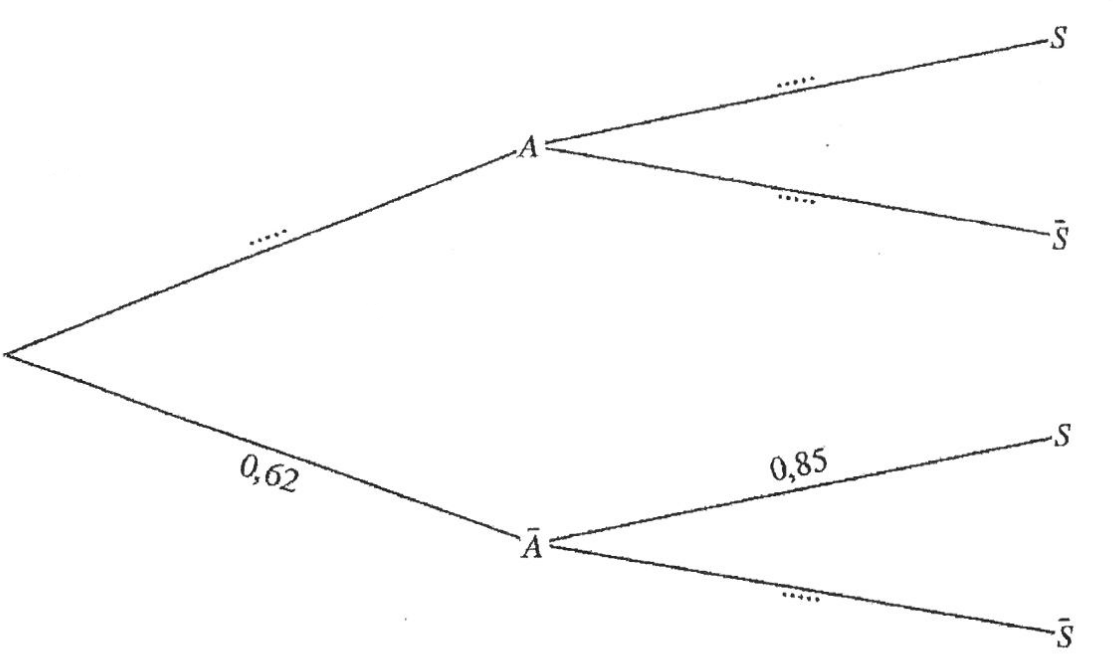
\includegraphics[width=\linewidth]{Arbuste.png}

\end{document}


 
